\documentclass[twoside]{book}

% Packages required by doxygen
\usepackage{fixltx2e}
\usepackage{calc}
\usepackage{doxygen}
\usepackage[export]{adjustbox} % also loads graphicx
\usepackage{graphicx}
\usepackage[utf8]{inputenc}
\usepackage{makeidx}
\usepackage{multicol}
\usepackage{multirow}
\PassOptionsToPackage{warn}{textcomp}
\usepackage{textcomp}
\usepackage[nointegrals]{wasysym}
\usepackage[table]{xcolor}

% Font selection
\usepackage[T1]{fontenc}
\usepackage[scaled=.90]{helvet}
\usepackage{courier}
\usepackage{amssymb}
\usepackage{sectsty}
\renewcommand{\familydefault}{\sfdefault}
\allsectionsfont{%
  \fontseries{bc}\selectfont%
  \color{darkgray}%
}
\renewcommand{\DoxyLabelFont}{%
  \fontseries{bc}\selectfont%
  \color{darkgray}%
}
\newcommand{\+}{\discretionary{\mbox{\scriptsize$\hookleftarrow$}}{}{}}

% Page & text layout
\usepackage{geometry}
\geometry{%
  a4paper,%
  top=2.5cm,%
  bottom=2.5cm,%
  left=2.5cm,%
  right=2.5cm%
}
\tolerance=750
\hfuzz=15pt
\hbadness=750
\setlength{\emergencystretch}{15pt}
\setlength{\parindent}{0cm}
\setlength{\parskip}{3ex plus 2ex minus 2ex}
\makeatletter
\renewcommand{\paragraph}{%
  \@startsection{paragraph}{4}{0ex}{-1.0ex}{1.0ex}{%
    \normalfont\normalsize\bfseries\SS@parafont%
  }%
}
\renewcommand{\subparagraph}{%
  \@startsection{subparagraph}{5}{0ex}{-1.0ex}{1.0ex}{%
    \normalfont\normalsize\bfseries\SS@subparafont%
  }%
}
\makeatother

% Headers & footers
\usepackage{fancyhdr}
\pagestyle{fancyplain}
\fancyhead[LE]{\fancyplain{}{\bfseries\thepage}}
\fancyhead[CE]{\fancyplain{}{}}
\fancyhead[RE]{\fancyplain{}{\bfseries\leftmark}}
\fancyhead[LO]{\fancyplain{}{\bfseries\rightmark}}
\fancyhead[CO]{\fancyplain{}{}}
\fancyhead[RO]{\fancyplain{}{\bfseries\thepage}}
\fancyfoot[LE]{\fancyplain{}{}}
\fancyfoot[CE]{\fancyplain{}{}}
\fancyfoot[RE]{\fancyplain{}{\bfseries\scriptsize Generated by Doxygen }}
\fancyfoot[LO]{\fancyplain{}{\bfseries\scriptsize Generated by Doxygen }}
\fancyfoot[CO]{\fancyplain{}{}}
\fancyfoot[RO]{\fancyplain{}{}}
\renewcommand{\footrulewidth}{0.4pt}
\renewcommand{\chaptermark}[1]{%
  \markboth{#1}{}%
}
\renewcommand{\sectionmark}[1]{%
  \markright{\thesection\ #1}%
}

% Indices & bibliography
\usepackage{natbib}
\usepackage[titles]{tocloft}
\setcounter{tocdepth}{3}
\setcounter{secnumdepth}{5}
\makeindex

% Hyperlinks (required, but should be loaded last)
\usepackage{ifpdf}
\ifpdf
  \usepackage[pdftex,pagebackref=true]{hyperref}
\else
  \usepackage[ps2pdf,pagebackref=true]{hyperref}
\fi
\hypersetup{%
  colorlinks=true,%
  linkcolor=blue,%
  citecolor=blue,%
  unicode%
}

% Custom commands
\newcommand{\clearemptydoublepage}{%
  \newpage{\pagestyle{empty}\cleardoublepage}%
}

\usepackage{caption}
\captionsetup{labelsep=space,justification=centering,font={bf},singlelinecheck=off,skip=4pt,position=top}

%===== C O N T E N T S =====

\begin{document}

% Titlepage & ToC
\hypersetup{pageanchor=false,
             bookmarksnumbered=true,
             pdfencoding=unicode
            }
\pagenumbering{roman}
\begin{titlepage}
\vspace*{7cm}
\begin{center}%
{\Large Foundit }\\
\vspace*{1cm}
{\large Generated by Doxygen 1.8.11}\\
\end{center}
\end{titlepage}
\clearemptydoublepage
\tableofcontents
\clearemptydoublepage
\pagenumbering{arabic}
\hypersetup{pageanchor=true}

%--- Begin generated contents ---
\chapter{Namespace Index}
\section{Namespace List}
Here is a list of all namespaces with brief descriptions\+:\begin{DoxyCompactList}
\item\contentsline{section}{\hyperlink{namespacefoundit}{foundit} }{\pageref{namespacefoundit}}{}
\item\contentsline{section}{\hyperlink{namespacefoundit_1_1admin}{foundit.\+admin} }{\pageref{namespacefoundit_1_1admin}}{}
\item\contentsline{section}{\hyperlink{namespacefoundit_1_1apps}{foundit.\+apps} }{\pageref{namespacefoundit_1_1apps}}{}
\item\contentsline{section}{\hyperlink{namespacefoundit_1_1foundit}{foundit.\+foundit} }{\pageref{namespacefoundit_1_1foundit}}{}
\item\contentsline{section}{\hyperlink{namespacefoundit_1_1foundit__old}{foundit.\+foundit\+\_\+old} }{\pageref{namespacefoundit_1_1foundit__old}}{}
\item\contentsline{section}{\hyperlink{namespacefoundit_1_1graph}{foundit.\+graph} }{\pageref{namespacefoundit_1_1graph}}{}
\item\contentsline{section}{\hyperlink{namespacefoundit_1_1graphtest}{foundit.\+graphtest} }{\pageref{namespacefoundit_1_1graphtest}}{}
\item\contentsline{section}{\hyperlink{namespacefoundit_1_1models}{foundit.\+models} }{\pageref{namespacefoundit_1_1models}}{}
\item\contentsline{section}{\hyperlink{namespacefoundit_1_1tests}{foundit.\+tests} }{\pageref{namespacefoundit_1_1tests}}{}
\item\contentsline{section}{\hyperlink{namespacefoundit_1_1urls}{foundit.\+urls} }{\pageref{namespacefoundit_1_1urls}}{}
\item\contentsline{section}{\hyperlink{namespacefoundit_1_1utils}{foundit.\+utils} }{\pageref{namespacefoundit_1_1utils}}{}
\item\contentsline{section}{\hyperlink{namespacefoundit_1_1views}{foundit.\+views} }{\pageref{namespacefoundit_1_1views}}{}
\end{DoxyCompactList}

\chapter{Hierarchical Index}
\section{Class Hierarchy}
This inheritance list is sorted roughly, but not completely, alphabetically\+:\begin{DoxyCompactList}
\item Model\begin{DoxyCompactList}
\item \contentsline{section}{foundit.\+models.\+Queuery}{\pageref{classfoundit_1_1models_1_1_queuery}}{}
\end{DoxyCompactList}
\item App\+Config\begin{DoxyCompactList}
\item \contentsline{section}{foundit.\+apps.\+Foundit\+Config}{\pageref{classfoundit_1_1apps_1_1_foundit_config}}{}
\end{DoxyCompactList}
\end{DoxyCompactList}

\chapter{Class Index}
\section{Class List}
Here are the classes, structs, unions and interfaces with brief descriptions\+:\begin{DoxyCompactList}
\item\contentsline{section}{\hyperlink{classfoundit_1_1apps_1_1_foundit_config}{foundit.\+apps.\+Foundit\+Config} }{\pageref{classfoundit_1_1apps_1_1_foundit_config}}{}
\item\contentsline{section}{\hyperlink{classfoundit_1_1models_1_1_queuery}{foundit.\+models.\+Queuery} }{\pageref{classfoundit_1_1models_1_1_queuery}}{}
\end{DoxyCompactList}

\chapter{File Index}
\section{File List}
Here is a list of all files with brief descriptions\+:\begin{DoxyCompactList}
\item\contentsline{section}{/home/user/\+Dropbox/\+School/\+C\+S\+C\+I Stuff/\+C\+S\+C\+I 3308-\/ Software Development/\+Foundit Project/ufoundit/foundit/\hyperlink{____init_____8py}{\+\_\+\+\_\+init\+\_\+\+\_\+.\+py} }{\pageref{____init_____8py}}{}
\item\contentsline{section}{/home/user/\+Dropbox/\+School/\+C\+S\+C\+I Stuff/\+C\+S\+C\+I 3308-\/ Software Development/\+Foundit Project/ufoundit/foundit/\hyperlink{admin_8py}{admin.\+py} }{\pageref{admin_8py}}{}
\item\contentsline{section}{/home/user/\+Dropbox/\+School/\+C\+S\+C\+I Stuff/\+C\+S\+C\+I 3308-\/ Software Development/\+Foundit Project/ufoundit/foundit/\hyperlink{apps_8py}{apps.\+py} }{\pageref{apps_8py}}{}
\item\contentsline{section}{/home/user/\+Dropbox/\+School/\+C\+S\+C\+I Stuff/\+C\+S\+C\+I 3308-\/ Software Development/\+Foundit Project/ufoundit/foundit/\hyperlink{foundit_8py}{foundit.\+py} }{\pageref{foundit_8py}}{}
\item\contentsline{section}{/home/user/\+Dropbox/\+School/\+C\+S\+C\+I Stuff/\+C\+S\+C\+I 3308-\/ Software Development/\+Foundit Project/ufoundit/foundit/\hyperlink{foundit__old_8py}{foundit\+\_\+old.\+py} }{\pageref{foundit__old_8py}}{}
\item\contentsline{section}{/home/user/\+Dropbox/\+School/\+C\+S\+C\+I Stuff/\+C\+S\+C\+I 3308-\/ Software Development/\+Foundit Project/ufoundit/foundit/\hyperlink{graph_8py}{graph.\+py} }{\pageref{graph_8py}}{}
\item\contentsline{section}{/home/user/\+Dropbox/\+School/\+C\+S\+C\+I Stuff/\+C\+S\+C\+I 3308-\/ Software Development/\+Foundit Project/ufoundit/foundit/\hyperlink{graphtest_8py}{graphtest.\+py} }{\pageref{graphtest_8py}}{}
\item\contentsline{section}{/home/user/\+Dropbox/\+School/\+C\+S\+C\+I Stuff/\+C\+S\+C\+I 3308-\/ Software Development/\+Foundit Project/ufoundit/foundit/\hyperlink{models_8py}{models.\+py} }{\pageref{models_8py}}{}
\item\contentsline{section}{/home/user/\+Dropbox/\+School/\+C\+S\+C\+I Stuff/\+C\+S\+C\+I 3308-\/ Software Development/\+Foundit Project/ufoundit/foundit/\hyperlink{tests_8py}{tests.\+py} }{\pageref{tests_8py}}{}
\item\contentsline{section}{/home/user/\+Dropbox/\+School/\+C\+S\+C\+I Stuff/\+C\+S\+C\+I 3308-\/ Software Development/\+Foundit Project/ufoundit/foundit/\hyperlink{urls_8py}{urls.\+py} }{\pageref{urls_8py}}{}
\item\contentsline{section}{/home/user/\+Dropbox/\+School/\+C\+S\+C\+I Stuff/\+C\+S\+C\+I 3308-\/ Software Development/\+Foundit Project/ufoundit/foundit/\hyperlink{utils_8py}{utils.\+py} }{\pageref{utils_8py}}{}
\item\contentsline{section}{/home/user/\+Dropbox/\+School/\+C\+S\+C\+I Stuff/\+C\+S\+C\+I 3308-\/ Software Development/\+Foundit Project/ufoundit/foundit/\hyperlink{views_8py}{views.\+py} }{\pageref{views_8py}}{}
\end{DoxyCompactList}

\chapter{Namespace Documentation}
\hypertarget{namespacefoundit}{}\section{foundit Namespace Reference}
\label{namespacefoundit}\index{foundit@{foundit}}
\subsection*{Namespaces}
\begin{DoxyCompactItemize}
\item 
 \hyperlink{namespacefoundit_1_1admin}{admin}
\item 
 \hyperlink{namespacefoundit_1_1apps}{apps}
\item 
 \hyperlink{namespacefoundit_1_1foundit}{foundit}
\item 
 \hyperlink{namespacefoundit_1_1foundit__old}{foundit\+\_\+old}
\item 
 \hyperlink{namespacefoundit_1_1graph}{graph}
\item 
 \hyperlink{namespacefoundit_1_1graphtest}{graphtest}
\item 
 \hyperlink{namespacefoundit_1_1models}{models}
\item 
 \hyperlink{namespacefoundit_1_1tests}{tests}
\item 
 \hyperlink{namespacefoundit_1_1urls}{urls}
\item 
 \hyperlink{namespacefoundit_1_1utils}{utils}
\item 
 \hyperlink{namespacefoundit_1_1views}{views}
\end{DoxyCompactItemize}

\hypertarget{namespacefoundit_1_1admin}{}\section{foundit.\+admin Namespace Reference}
\label{namespacefoundit_1_1admin}\index{foundit.\+admin@{foundit.\+admin}}

\hypertarget{namespacefoundit_1_1apps}{}\section{foundit.\+apps Namespace Reference}
\label{namespacefoundit_1_1apps}\index{foundit.\+apps@{foundit.\+apps}}
\subsection*{Classes}
\begin{DoxyCompactItemize}
\item 
class \hyperlink{classfoundit_1_1apps_1_1_foundit_config}{Foundit\+Config}
\end{DoxyCompactItemize}

\hypertarget{namespacefoundit_1_1foundit}{}\section{foundit.\+foundit Namespace Reference}
\label{namespacefoundit_1_1foundit}\index{foundit.\+foundit@{foundit.\+foundit}}
\subsection*{Functions}
\begin{DoxyCompactItemize}
\item 
def \hyperlink{namespacefoundit_1_1foundit_a417cf87b2677c1439ee12bab5e23124e}{schedule} (subreddit, post\+Limit, top\+Com\+Limit, top\+Reply\+Limit, top\+Word\+Limit, top\+User\+Limit, oldest\+Post\+Limit, active\+Post\+Limit, wc)
\item 
def \hyperlink{namespacefoundit_1_1foundit_a8904e5a32351d54fbbc0971b30424e6c}{get\+Submission\+Age} (submission)
\begin{DoxyCompactList}\small\item\em temp=q.\+fetch\+\_\+job(jobq\mbox{[}qindex\mbox{]}).get\+\_\+id.\+result temp=q.\+fetch\+\_\+job(jobq\mbox{[}qindex\mbox{]}).id.\+result if(temp)\+: results.\+append(temp) q.\+remove(q.\+fetch\+\_\+job(jobq\mbox{[}qindex\mbox{]}).id) check+=1 gindex+=1 print(\char`\"{}\+W\+O\+R\+K\+E\+R S\+E\+A\+R\+C\+H \#\char`\"{}+str(qindex)+(\char`\"{} D\+O\+N\+E!!!\char`\"{})+\char`\"{}v\+T\+O\+T\+A\+L C\+O\+M\+P\+L\+E\+T\+E\+: \char`\"{}+str(check)) time.\+sleep(workercount+3) qindex+=1 time.\+sleep(workercount$\ast$2) print(\char`\"{}\+W\+A\+I\+T\+I\+N\+G...\char`\"{}) if(check!=workercount)\+: qindex=0 C\+O\+M\+B\+I\+NE A\+LL D\+A\+TA O\+N\+CE C\+H\+E\+CK P\+A\+S\+S\+ES O\+R\+D\+ER OF R\+E\+T\+U\+RN F\+OR W\+O\+R\+K\+E\+RS 0title\+Words, 1noun\+Dict, 2user\+Dict, 3top\+Com, 4top\+Reply, 5oldest\+Post, 6active\+Post, 7posts\+Analyzed, 8total\+Length\+All, 9comments\+Analyzed) \end{DoxyCompactList}\item 
def \hyperlink{namespacefoundit_1_1foundit_ae5d1e300e19274d4bb4c0db668d13714}{adjust} (l, limit, index\+To\+Compare, thing\+To\+Add)
\item 
def \hyperlink{namespacefoundit_1_1foundit_a0a97ddadcb8a2cc47d44c8810dc8af05}{search} (subreddit, post\+Limit, top\+Com\+Limit, top\+Reply\+Limit, top\+Word\+Limit, top\+User\+Limit, oldest\+Post\+Limit, active\+Post\+Limit, startpos, endpos, qindex)
\end{DoxyCompactItemize}
\subsection*{Variables}
\begin{DoxyCompactItemize}
\item 
\hyperlink{namespacefoundit_1_1foundit_ae9cda1f3b56d2dd4499216536e44b722}{q} = Queue(connection=conn)
\end{DoxyCompactItemize}


\subsection{Function Documentation}
\index{foundit\+::foundit@{foundit\+::foundit}!adjust@{adjust}}
\index{adjust@{adjust}!foundit\+::foundit@{foundit\+::foundit}}
\subsubsection[{\texorpdfstring{adjust(l, limit, index\+To\+Compare, thing\+To\+Add)}{adjust(l, limit, indexToCompare, thingToAdd)}}]{\setlength{\rightskip}{0pt plus 5cm}def foundit.\+foundit.\+adjust (
\begin{DoxyParamCaption}
\item[{}]{l, }
\item[{}]{limit, }
\item[{}]{index\+To\+Compare, }
\item[{}]{thing\+To\+Add}
\end{DoxyParamCaption}
)}\hypertarget{namespacefoundit_1_1foundit_ae5d1e300e19274d4bb4c0db668d13714}{}\label{namespacefoundit_1_1foundit_ae5d1e300e19274d4bb4c0db668d13714}
\begin{DoxyVerb}The adjust function is responsible for the handling of the word graph. It first fills a list of words to compare which the lowest value is popped off in exchange for another word to add. 
\end{DoxyVerb}
 \index{foundit\+::foundit@{foundit\+::foundit}!get\+Submission\+Age@{get\+Submission\+Age}}
\index{get\+Submission\+Age@{get\+Submission\+Age}!foundit\+::foundit@{foundit\+::foundit}}
\subsubsection[{\texorpdfstring{get\+Submission\+Age(submission)}{getSubmissionAge(submission)}}]{\setlength{\rightskip}{0pt plus 5cm}def foundit.\+foundit.\+get\+Submission\+Age (
\begin{DoxyParamCaption}
\item[{}]{submission}
\end{DoxyParamCaption}
)}\hypertarget{namespacefoundit_1_1foundit_a8904e5a32351d54fbbc0971b30424e6c}{}\label{namespacefoundit_1_1foundit_a8904e5a32351d54fbbc0971b30424e6c}


temp=q.\+fetch\+\_\+job(jobq\mbox{[}qindex\mbox{]}).get\+\_\+id.\+result temp=q.\+fetch\+\_\+job(jobq\mbox{[}qindex\mbox{]}).id.\+result if(temp)\+: results.\+append(temp) q.\+remove(q.\+fetch\+\_\+job(jobq\mbox{[}qindex\mbox{]}).id) check+=1 gindex+=1 print(\char`\"{}\+W\+O\+R\+K\+E\+R S\+E\+A\+R\+C\+H \#\char`\"{}+str(qindex)+(\char`\"{} D\+O\+N\+E!!!\char`\"{})+\char`\"{}v\+T\+O\+T\+A\+L C\+O\+M\+P\+L\+E\+T\+E\+: \char`\"{}+str(check)) time.\+sleep(workercount+3) qindex+=1 time.\+sleep(workercount$\ast$2) print(\char`\"{}\+W\+A\+I\+T\+I\+N\+G...\char`\"{}) if(check!=workercount)\+: qindex=0 C\+O\+M\+B\+I\+NE A\+LL D\+A\+TA O\+N\+CE C\+H\+E\+CK P\+A\+S\+S\+ES O\+R\+D\+ER OF R\+E\+T\+U\+RN F\+OR W\+O\+R\+K\+E\+RS 0title\+Words, 1noun\+Dict, 2user\+Dict, 3top\+Com, 4top\+Reply, 5oldest\+Post, 6active\+Post, 7posts\+Analyzed, 8total\+Length\+All, 9comments\+Analyzed) 

\begin{DoxyVerb}This function gets the age of the current submission based on the comparision between the submission time and the current time. 
\end{DoxyVerb}
 \index{foundit\+::foundit@{foundit\+::foundit}!schedule@{schedule}}
\index{schedule@{schedule}!foundit\+::foundit@{foundit\+::foundit}}
\subsubsection[{\texorpdfstring{schedule(subreddit, post\+Limit, top\+Com\+Limit, top\+Reply\+Limit, top\+Word\+Limit, top\+User\+Limit, oldest\+Post\+Limit, active\+Post\+Limit, wc)}{schedule(subreddit, postLimit, topComLimit, topReplyLimit, topWordLimit, topUserLimit, oldestPostLimit, activePostLimit, wc)}}]{\setlength{\rightskip}{0pt plus 5cm}def foundit.\+foundit.\+schedule (
\begin{DoxyParamCaption}
\item[{}]{subreddit, }
\item[{}]{post\+Limit, }
\item[{}]{top\+Com\+Limit, }
\item[{}]{top\+Reply\+Limit, }
\item[{}]{top\+Word\+Limit, }
\item[{}]{top\+User\+Limit, }
\item[{}]{oldest\+Post\+Limit, }
\item[{}]{active\+Post\+Limit, }
\item[{}]{wc}
\end{DoxyParamCaption}
)}\hypertarget{namespacefoundit_1_1foundit_a417cf87b2677c1439ee12bab5e23124e}{}\label{namespacefoundit_1_1foundit_a417cf87b2677c1439ee12bab5e23124e}
\begin{DoxyVerb}The schedule function is responsible for scheduling worker jobs. These workers will divide the total work time amongst themselves to decrease the time of the search and compiling of Foundit.
\end{DoxyVerb}
 \index{foundit\+::foundit@{foundit\+::foundit}!search@{search}}
\index{search@{search}!foundit\+::foundit@{foundit\+::foundit}}
\subsubsection[{\texorpdfstring{search(subreddit, post\+Limit, top\+Com\+Limit, top\+Reply\+Limit, top\+Word\+Limit, top\+User\+Limit, oldest\+Post\+Limit, active\+Post\+Limit, startpos, endpos, qindex)}{search(subreddit, postLimit, topComLimit, topReplyLimit, topWordLimit, topUserLimit, oldestPostLimit, activePostLimit, startpos, endpos, qindex)}}]{\setlength{\rightskip}{0pt plus 5cm}def foundit.\+foundit.\+search (
\begin{DoxyParamCaption}
\item[{}]{subreddit, }
\item[{}]{post\+Limit, }
\item[{}]{top\+Com\+Limit, }
\item[{}]{top\+Reply\+Limit, }
\item[{}]{top\+Word\+Limit, }
\item[{}]{top\+User\+Limit, }
\item[{}]{oldest\+Post\+Limit, }
\item[{}]{active\+Post\+Limit, }
\item[{}]{startpos, }
\item[{}]{endpos, }
\item[{}]{qindex}
\end{DoxyParamCaption}
)}\hypertarget{namespacefoundit_1_1foundit_a0a97ddadcb8a2cc47d44c8810dc8af05}{}\label{namespacefoundit_1_1foundit_a0a97ddadcb8a2cc47d44c8810dc8af05}
\begin{DoxyVerb}The search function is responsible for gathering and parsing the reddit data for further use. It also uses the language tool NLTK to create a working dictionary for the found words to be passed through. This also alleviates the need to worry about common words such as "the" or "a".  The function then returns parsed reddit data ready for further use.
\end{DoxyVerb}
 

\subsection{Variable Documentation}
\index{foundit\+::foundit@{foundit\+::foundit}!q@{q}}
\index{q@{q}!foundit\+::foundit@{foundit\+::foundit}}
\subsubsection[{\texorpdfstring{q}{q}}]{\setlength{\rightskip}{0pt plus 5cm}foundit.\+foundit.\+q = Queue(connection=conn)}\hypertarget{namespacefoundit_1_1foundit_ae9cda1f3b56d2dd4499216536e44b722}{}\label{namespacefoundit_1_1foundit_ae9cda1f3b56d2dd4499216536e44b722}

\hypertarget{namespacefoundit_1_1foundit__old}{}\section{foundit.\+foundit\+\_\+old Namespace Reference}
\label{namespacefoundit_1_1foundit__old}\index{foundit.\+foundit\+\_\+old@{foundit.\+foundit\+\_\+old}}
\subsection*{Functions}
\begin{DoxyCompactItemize}
\item 
def \hyperlink{namespacefoundit_1_1foundit__old_a87bf8701c89694eb3f6c6fbd11582ff5}{get\+Submission\+Age} (submission)
\item 
def \hyperlink{namespacefoundit_1_1foundit__old_ab326b5587621f5ce27348998be899ff6}{search} (subreddit, post\+Limit, top\+Com\+Limit, top\+Word\+Limit, top\+User\+Limit, oh\+Snap\+Limit, oldest\+Post\+Limit)
\end{DoxyCompactItemize}


\subsection{Function Documentation}
\index{foundit\+::foundit\+\_\+old@{foundit\+::foundit\+\_\+old}!get\+Submission\+Age@{get\+Submission\+Age}}
\index{get\+Submission\+Age@{get\+Submission\+Age}!foundit\+::foundit\+\_\+old@{foundit\+::foundit\+\_\+old}}
\subsubsection[{\texorpdfstring{get\+Submission\+Age(submission)}{getSubmissionAge(submission)}}]{\setlength{\rightskip}{0pt plus 5cm}def foundit.\+foundit\+\_\+old.\+get\+Submission\+Age (
\begin{DoxyParamCaption}
\item[{}]{submission}
\end{DoxyParamCaption}
)}\hypertarget{namespacefoundit_1_1foundit__old_a87bf8701c89694eb3f6c6fbd11582ff5}{}\label{namespacefoundit_1_1foundit__old_a87bf8701c89694eb3f6c6fbd11582ff5}
\index{foundit\+::foundit\+\_\+old@{foundit\+::foundit\+\_\+old}!search@{search}}
\index{search@{search}!foundit\+::foundit\+\_\+old@{foundit\+::foundit\+\_\+old}}
\subsubsection[{\texorpdfstring{search(subreddit, post\+Limit, top\+Com\+Limit, top\+Word\+Limit, top\+User\+Limit, oh\+Snap\+Limit, oldest\+Post\+Limit)}{search(subreddit, postLimit, topComLimit, topWordLimit, topUserLimit, ohSnapLimit, oldestPostLimit)}}]{\setlength{\rightskip}{0pt plus 5cm}def foundit.\+foundit\+\_\+old.\+search (
\begin{DoxyParamCaption}
\item[{}]{subreddit, }
\item[{}]{post\+Limit, }
\item[{}]{top\+Com\+Limit, }
\item[{}]{top\+Word\+Limit, }
\item[{}]{top\+User\+Limit, }
\item[{}]{oh\+Snap\+Limit, }
\item[{}]{oldest\+Post\+Limit}
\end{DoxyParamCaption}
)}\hypertarget{namespacefoundit_1_1foundit__old_ab326b5587621f5ce27348998be899ff6}{}\label{namespacefoundit_1_1foundit__old_ab326b5587621f5ce27348998be899ff6}

\hypertarget{namespacefoundit_1_1graph}{}\section{foundit.\+graph Namespace Reference}
\label{namespacefoundit_1_1graph}\index{foundit.\+graph@{foundit.\+graph}}
\subsection*{Functions}
\begin{DoxyCompactItemize}
\item 
def \hyperlink{namespacefoundit_1_1graph_ad382cb5cac25f52e045b61c77b3e5245}{uautolabel} (rects, ax)
\item 
def \hyperlink{namespacefoundit_1_1graph_ac72321993b1a3abe0633ffb1f3ac4d08}{urender\+Graph} (data\+Set)
\item 
def \hyperlink{namespacefoundit_1_1graph_a831dedc0a3b858f3c05ef6e19d45667f}{render\+Graph} (data\+Set)
\end{DoxyCompactItemize}


\subsection{Function Documentation}
\index{foundit\+::graph@{foundit\+::graph}!render\+Graph@{render\+Graph}}
\index{render\+Graph@{render\+Graph}!foundit\+::graph@{foundit\+::graph}}
\subsubsection[{\texorpdfstring{render\+Graph(data\+Set)}{renderGraph(dataSet)}}]{\setlength{\rightskip}{0pt plus 5cm}def foundit.\+graph.\+render\+Graph (
\begin{DoxyParamCaption}
\item[{}]{data\+Set}
\end{DoxyParamCaption}
)}\hypertarget{namespacefoundit_1_1graph_a831dedc0a3b858f3c05ef6e19d45667f}{}\label{namespacefoundit_1_1graph_a831dedc0a3b858f3c05ef6e19d45667f}
\begin{DoxyVerb}The renderGraph function converts data into a bar graph object. It handles the measuring, drawing, and defining of the various aspects of the graph. From this point, it converts the graph code from Python to HTML and returns this value. This HTML code is then transferred to the website for the viewer.
\end{DoxyVerb}
 \index{foundit\+::graph@{foundit\+::graph}!uautolabel@{uautolabel}}
\index{uautolabel@{uautolabel}!foundit\+::graph@{foundit\+::graph}}
\subsubsection[{\texorpdfstring{uautolabel(rects, ax)}{uautolabel(rects, ax)}}]{\setlength{\rightskip}{0pt plus 5cm}def foundit.\+graph.\+uautolabel (
\begin{DoxyParamCaption}
\item[{}]{rects, }
\item[{}]{ax}
\end{DoxyParamCaption}
)}\hypertarget{namespacefoundit_1_1graph_ad382cb5cac25f52e045b61c77b3e5245}{}\label{namespacefoundit_1_1graph_ad382cb5cac25f52e045b61c77b3e5245}
\begin{DoxyVerb}Function attaches a text label above each bar displaying its height. This function provides the reader easy context on each value in the finished graph so that an understanding of the data can be made faster.
\end{DoxyVerb}
 \index{foundit\+::graph@{foundit\+::graph}!urender\+Graph@{urender\+Graph}}
\index{urender\+Graph@{urender\+Graph}!foundit\+::graph@{foundit\+::graph}}
\subsubsection[{\texorpdfstring{urender\+Graph(data\+Set)}{urenderGraph(dataSet)}}]{\setlength{\rightskip}{0pt plus 5cm}def foundit.\+graph.\+urender\+Graph (
\begin{DoxyParamCaption}
\item[{}]{data\+Set}
\end{DoxyParamCaption}
)}\hypertarget{namespacefoundit_1_1graph_ac72321993b1a3abe0633ffb1f3ac4d08}{}\label{namespacefoundit_1_1graph_ac72321993b1a3abe0633ffb1f3ac4d08}
\begin{DoxyVerb}This function renders a graph for the use in the specialized word graphs. This portion of the code was not completed at the time of submission, and so this function is currently not being used. 
\end{DoxyVerb}
 
\hypertarget{namespacefoundit_1_1graphtest}{}\section{foundit.\+graphtest Namespace Reference}
\label{namespacefoundit_1_1graphtest}\index{foundit.\+graphtest@{foundit.\+graphtest}}
\subsection*{Variables}
\begin{DoxyCompactItemize}
\item 
list \hyperlink{namespacefoundit_1_1graphtest_a598db4fa9693ae9cc94d8ebe41d59224}{a} = \mbox{[}1, 2\mbox{]}
\item 
list \hyperlink{namespacefoundit_1_1graphtest_add8d87bd6a6890fe6f2682f0f7990ed9}{b} = \mbox{[}2, 5\mbox{]}
\item 
\hyperlink{namespacefoundit_1_1graphtest_aae9ec7ea98940dc46b73c2908419e44c}{bins}
\item 
\hyperlink{namespacefoundit_1_1graphtest_a0717e136db67aedb0ff4cffd4fc30c5f}{weights}
\end{DoxyCompactItemize}


\subsection{Variable Documentation}
\index{foundit\+::graphtest@{foundit\+::graphtest}!a@{a}}
\index{a@{a}!foundit\+::graphtest@{foundit\+::graphtest}}
\subsubsection[{\texorpdfstring{a}{a}}]{\setlength{\rightskip}{0pt plus 5cm}foundit.\+graphtest.\+a = \mbox{[}1, 2\mbox{]}}\hypertarget{namespacefoundit_1_1graphtest_a598db4fa9693ae9cc94d8ebe41d59224}{}\label{namespacefoundit_1_1graphtest_a598db4fa9693ae9cc94d8ebe41d59224}
\index{foundit\+::graphtest@{foundit\+::graphtest}!b@{b}}
\index{b@{b}!foundit\+::graphtest@{foundit\+::graphtest}}
\subsubsection[{\texorpdfstring{b}{b}}]{\setlength{\rightskip}{0pt plus 5cm}list foundit.\+graphtest.\+b = \mbox{[}2, 5\mbox{]}}\hypertarget{namespacefoundit_1_1graphtest_add8d87bd6a6890fe6f2682f0f7990ed9}{}\label{namespacefoundit_1_1graphtest_add8d87bd6a6890fe6f2682f0f7990ed9}
\index{foundit\+::graphtest@{foundit\+::graphtest}!bins@{bins}}
\index{bins@{bins}!foundit\+::graphtest@{foundit\+::graphtest}}
\subsubsection[{\texorpdfstring{bins}{bins}}]{\setlength{\rightskip}{0pt plus 5cm}foundit.\+graphtest.\+bins}\hypertarget{namespacefoundit_1_1graphtest_aae9ec7ea98940dc46b73c2908419e44c}{}\label{namespacefoundit_1_1graphtest_aae9ec7ea98940dc46b73c2908419e44c}
\index{foundit\+::graphtest@{foundit\+::graphtest}!weights@{weights}}
\index{weights@{weights}!foundit\+::graphtest@{foundit\+::graphtest}}
\subsubsection[{\texorpdfstring{weights}{weights}}]{\setlength{\rightskip}{0pt plus 5cm}foundit.\+graphtest.\+weights}\hypertarget{namespacefoundit_1_1graphtest_a0717e136db67aedb0ff4cffd4fc30c5f}{}\label{namespacefoundit_1_1graphtest_a0717e136db67aedb0ff4cffd4fc30c5f}

\hypertarget{namespacefoundit_1_1models}{}\section{foundit.\+models Namespace Reference}
\label{namespacefoundit_1_1models}\index{foundit.\+models@{foundit.\+models}}
\subsection*{Classes}
\begin{DoxyCompactItemize}
\item 
class \hyperlink{classfoundit_1_1models_1_1_queuery}{Queuery}
\end{DoxyCompactItemize}

\hypertarget{namespacefoundit_1_1tests}{}\section{foundit.\+tests Namespace Reference}
\label{namespacefoundit_1_1tests}\index{foundit.\+tests@{foundit.\+tests}}

\hypertarget{namespacefoundit_1_1urls}{}\section{foundit.\+urls Namespace Reference}
\label{namespacefoundit_1_1urls}\index{foundit.\+urls@{foundit.\+urls}}
\subsection*{Variables}
\begin{DoxyCompactItemize}
\item 
list \hyperlink{namespacefoundit_1_1urls_aa83b5e06599a5865f06d3d9c2d4f5a21}{urlpatterns}
\end{DoxyCompactItemize}


\subsection{Variable Documentation}
\index{foundit\+::urls@{foundit\+::urls}!urlpatterns@{urlpatterns}}
\index{urlpatterns@{urlpatterns}!foundit\+::urls@{foundit\+::urls}}
\subsubsection[{\texorpdfstring{urlpatterns}{urlpatterns}}]{\setlength{\rightskip}{0pt plus 5cm}list foundit.\+urls.\+urlpatterns}\hypertarget{namespacefoundit_1_1urls_aa83b5e06599a5865f06d3d9c2d4f5a21}{}\label{namespacefoundit_1_1urls_aa83b5e06599a5865f06d3d9c2d4f5a21}
{\bfseries Initial value\+:}
\begin{DoxyCode}
1 = [
2     url(\textcolor{stringliteral}{r'^$'}, views.index, name=\textcolor{stringliteral}{'index'}),
3     url(\textcolor{stringliteral}{r'^results/$'}, views.results, name=\textcolor{stringliteral}{'results'}),
4     url(\textcolor{stringliteral}{r'^loading/$'}, views.loading, name=\textcolor{stringliteral}{'loading'}),
5     url(\textcolor{stringliteral}{r'^loading/checkJob'}, views.checkJob, name=\textcolor{stringliteral}{'checkJob'}),
6     url(\textcolor{stringliteral}{r'^testResults/$'}, views.testResults, name=\textcolor{stringliteral}{'testResults'}),
7 ]
\end{DoxyCode}

\hypertarget{namespacefoundit_1_1utils}{}\section{foundit.\+utils Namespace Reference}
\label{namespacefoundit_1_1utils}\index{foundit.\+utils@{foundit.\+utils}}
\subsection*{Functions}
\begin{DoxyCompactItemize}
\item 
def \hyperlink{namespacefoundit_1_1utils_a59497bd850949eb6946d3ddf7fb17d85}{return\+U\+RL} (str1, str2)
\end{DoxyCompactItemize}


\subsection{Function Documentation}
\index{foundit\+::utils@{foundit\+::utils}!return\+U\+RL@{return\+U\+RL}}
\index{return\+U\+RL@{return\+U\+RL}!foundit\+::utils@{foundit\+::utils}}
\subsubsection[{\texorpdfstring{return\+U\+R\+L(str1, str2)}{returnURL(str1, str2)}}]{\setlength{\rightskip}{0pt plus 5cm}def foundit.\+utils.\+return\+U\+RL (
\begin{DoxyParamCaption}
\item[{}]{str1, }
\item[{}]{str2}
\end{DoxyParamCaption}
)}\hypertarget{namespacefoundit_1_1utils_a59497bd850949eb6946d3ddf7fb17d85}{}\label{namespacefoundit_1_1utils_a59497bd850949eb6946d3ddf7fb17d85}
\begin{DoxyVerb}combine strings into full URL
\end{DoxyVerb}
 
\hypertarget{namespacefoundit_1_1views}{}\section{foundit.\+views Namespace Reference}
\label{namespacefoundit_1_1views}\index{foundit.\+views@{foundit.\+views}}
\subsection*{Functions}
\begin{DoxyCompactItemize}
\item 
def \hyperlink{namespacefoundit_1_1views_a7dd28e8760cb6ba397d734043c840841}{index} (request)
\item 
def \hyperlink{namespacefoundit_1_1views_a1cea187af3aaa9ac41218cd985a3f24b}{loading} (request)
\item 
def \hyperlink{namespacefoundit_1_1views_a91bc63c48fad0582cbcff41458970486}{check\+Job} (request)
\item 
def \hyperlink{namespacefoundit_1_1views_a07ba7672a02678833190150670718cae}{test\+Results} (request)
\item 
def \hyperlink{namespacefoundit_1_1views_aaacc45f037dbadfc5ecd92f0a1ffa4e6}{results} (request)
\end{DoxyCompactItemize}
\subsection*{Variables}
\begin{DoxyCompactItemize}
\item 
\hyperlink{namespacefoundit_1_1views_a933f4b14aa78ea94e74f8f93970e4b12}{q} = Queue(connection=conn)
\item 
string \hyperlink{namespacefoundit_1_1views_a326af97fa9bba95a26dcbb7c1a1f0f04}{title} = \char`\"{}\char`\"{}
\item 
int \hyperlink{namespacefoundit_1_1views_adcdd2d7a86d9c9a1d91112a22adab904}{workercount} = 5
\end{DoxyCompactItemize}


\subsection{Function Documentation}
\index{foundit\+::views@{foundit\+::views}!check\+Job@{check\+Job}}
\index{check\+Job@{check\+Job}!foundit\+::views@{foundit\+::views}}
\subsubsection[{\texorpdfstring{check\+Job(request)}{checkJob(request)}}]{\setlength{\rightskip}{0pt plus 5cm}def foundit.\+views.\+check\+Job (
\begin{DoxyParamCaption}
\item[{}]{request}
\end{DoxyParamCaption}
)}\hypertarget{namespacefoundit_1_1views_a91bc63c48fad0582cbcff41458970486}{}\label{namespacefoundit_1_1views_a91bc63c48fad0582cbcff41458970486}
\begin{DoxyVerb}This function requests the jobid of a reddit instance that was established in loading. From this point, it returns an html object of either the jobid or the existing job with that id.     
\end{DoxyVerb}
 \index{foundit\+::views@{foundit\+::views}!index@{index}}
\index{index@{index}!foundit\+::views@{foundit\+::views}}
\subsubsection[{\texorpdfstring{index(request)}{index(request)}}]{\setlength{\rightskip}{0pt plus 5cm}def foundit.\+views.\+index (
\begin{DoxyParamCaption}
\item[{}]{request}
\end{DoxyParamCaption}
)}\hypertarget{namespacefoundit_1_1views_a7dd28e8760cb6ba397d734043c840841}{}\label{namespacefoundit_1_1views_a7dd28e8760cb6ba397d734043c840841}
\begin{DoxyVerb}The index function establishes connection to the index of website.
\end{DoxyVerb}
 \index{foundit\+::views@{foundit\+::views}!loading@{loading}}
\index{loading@{loading}!foundit\+::views@{foundit\+::views}}
\subsubsection[{\texorpdfstring{loading(request)}{loading(request)}}]{\setlength{\rightskip}{0pt plus 5cm}def foundit.\+views.\+loading (
\begin{DoxyParamCaption}
\item[{}]{request}
\end{DoxyParamCaption}
)}\hypertarget{namespacefoundit_1_1views_a1cea187af3aaa9ac41218cd985a3f24b}{}\label{namespacefoundit_1_1views_a1cea187af3aaa9ac41218cd985a3f24b}
\begin{DoxyVerb}The loading function is responsible for requesting a reddit instance and gathering the various data from it. From that point, it adds these values to a list and saves this as a job. Then the function establishes a context for the instance which is made from the current job id and subreddit values. Finally, this function returns the rendering of the context.
\end{DoxyVerb}
 \index{foundit\+::views@{foundit\+::views}!results@{results}}
\index{results@{results}!foundit\+::views@{foundit\+::views}}
\subsubsection[{\texorpdfstring{results(request)}{results(request)}}]{\setlength{\rightskip}{0pt plus 5cm}def foundit.\+views.\+results (
\begin{DoxyParamCaption}
\item[{}]{request}
\end{DoxyParamCaption}
)}\hypertarget{namespacefoundit_1_1views_aaacc45f037dbadfc5ecd92f0a1ffa4e6}{}\label{namespacefoundit_1_1views_aaacc45f037dbadfc5ecd92f0a1ffa4e6}
\begin{DoxyVerb}This function is responsible for parsing the data from reddit into appropriate variables.
Additionally, it passes this data into graphing functions for its later use in providing result-based graphs on the website.
Results also returns the context variable which contains the necessary data for later construction of the website. 
This function provides the heavy lifting of Foundit, as it provides the data used for the later analtyics. 
\end{DoxyVerb}
 \index{foundit\+::views@{foundit\+::views}!test\+Results@{test\+Results}}
\index{test\+Results@{test\+Results}!foundit\+::views@{foundit\+::views}}
\subsubsection[{\texorpdfstring{test\+Results(request)}{testResults(request)}}]{\setlength{\rightskip}{0pt plus 5cm}def foundit.\+views.\+test\+Results (
\begin{DoxyParamCaption}
\item[{}]{request}
\end{DoxyParamCaption}
)}\hypertarget{namespacefoundit_1_1views_a07ba7672a02678833190150670718cae}{}\label{namespacefoundit_1_1views_a07ba7672a02678833190150670718cae}
\begin{DoxyVerb}This function's purpose is to return an html response of results. This was a test function?
\end{DoxyVerb}
 

\subsection{Variable Documentation}
\index{foundit\+::views@{foundit\+::views}!q@{q}}
\index{q@{q}!foundit\+::views@{foundit\+::views}}
\subsubsection[{\texorpdfstring{q}{q}}]{\setlength{\rightskip}{0pt plus 5cm}foundit.\+views.\+q = Queue(connection=conn)}\hypertarget{namespacefoundit_1_1views_a933f4b14aa78ea94e74f8f93970e4b12}{}\label{namespacefoundit_1_1views_a933f4b14aa78ea94e74f8f93970e4b12}
\index{foundit\+::views@{foundit\+::views}!title@{title}}
\index{title@{title}!foundit\+::views@{foundit\+::views}}
\subsubsection[{\texorpdfstring{title}{title}}]{\setlength{\rightskip}{0pt plus 5cm}string foundit.\+views.\+title = \char`\"{}\char`\"{}}\hypertarget{namespacefoundit_1_1views_a326af97fa9bba95a26dcbb7c1a1f0f04}{}\label{namespacefoundit_1_1views_a326af97fa9bba95a26dcbb7c1a1f0f04}
\index{foundit\+::views@{foundit\+::views}!workercount@{workercount}}
\index{workercount@{workercount}!foundit\+::views@{foundit\+::views}}
\subsubsection[{\texorpdfstring{workercount}{workercount}}]{\setlength{\rightskip}{0pt plus 5cm}int foundit.\+views.\+workercount = 5}\hypertarget{namespacefoundit_1_1views_adcdd2d7a86d9c9a1d91112a22adab904}{}\label{namespacefoundit_1_1views_adcdd2d7a86d9c9a1d91112a22adab904}

\chapter{Class Documentation}
\hypertarget{classfoundit_1_1apps_1_1_foundit_config}{}\section{foundit.\+apps.\+Foundit\+Config Class Reference}
\label{classfoundit_1_1apps_1_1_foundit_config}\index{foundit.\+apps.\+Foundit\+Config@{foundit.\+apps.\+Foundit\+Config}}


Inheritance diagram for foundit.\+apps.\+Foundit\+Config\+:\nopagebreak
\begin{figure}[H]
\begin{center}
\leavevmode
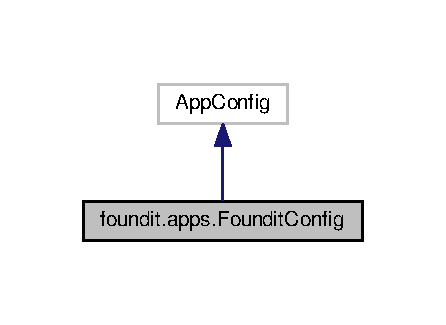
\includegraphics[width=214pt]{classfoundit_1_1apps_1_1_foundit_config__inherit__graph}
\end{center}
\end{figure}


Collaboration diagram for foundit.\+apps.\+Foundit\+Config\+:\nopagebreak
\begin{figure}[H]
\begin{center}
\leavevmode
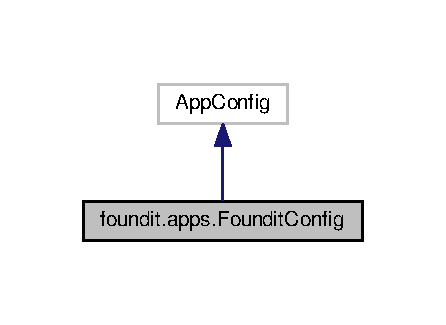
\includegraphics[width=214pt]{classfoundit_1_1apps_1_1_foundit_config__coll__graph}
\end{center}
\end{figure}
\subsection*{Static Public Attributes}
\begin{DoxyCompactItemize}
\item 
string \hyperlink{classfoundit_1_1apps_1_1_foundit_config_a6acdf3587456db7401bd4701743c6b9d}{name} = \textquotesingle{}foundit\textquotesingle{}
\end{DoxyCompactItemize}


\subsection{Member Data Documentation}
\index{foundit\+::apps\+::\+Foundit\+Config@{foundit\+::apps\+::\+Foundit\+Config}!name@{name}}
\index{name@{name}!foundit\+::apps\+::\+Foundit\+Config@{foundit\+::apps\+::\+Foundit\+Config}}
\subsubsection[{\texorpdfstring{name}{name}}]{\setlength{\rightskip}{0pt plus 5cm}string foundit.\+apps.\+Foundit\+Config.\+name = \textquotesingle{}foundit\textquotesingle{}\hspace{0.3cm}{\ttfamily [static]}}\hypertarget{classfoundit_1_1apps_1_1_foundit_config_a6acdf3587456db7401bd4701743c6b9d}{}\label{classfoundit_1_1apps_1_1_foundit_config_a6acdf3587456db7401bd4701743c6b9d}


The documentation for this class was generated from the following file\+:\begin{DoxyCompactItemize}
\item 
/home/user/\+Dropbox/\+School/\+C\+S\+C\+I Stuff/\+C\+S\+C\+I 3308-\/ Software Development/\+Foundit Project/ufoundit/foundit/\hyperlink{apps_8py}{apps.\+py}\end{DoxyCompactItemize}

\hypertarget{classfoundit_1_1models_1_1_queuery}{}\section{foundit.\+models.\+Queuery Class Reference}
\label{classfoundit_1_1models_1_1_queuery}\index{foundit.\+models.\+Queuery@{foundit.\+models.\+Queuery}}


Inheritance diagram for foundit.\+models.\+Queuery\+:\nopagebreak
\begin{figure}[H]
\begin{center}
\leavevmode
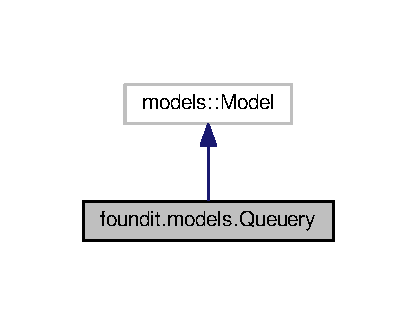
\includegraphics[width=200pt]{classfoundit_1_1models_1_1_queuery__inherit__graph}
\end{center}
\end{figure}


Collaboration diagram for foundit.\+models.\+Queuery\+:\nopagebreak
\begin{figure}[H]
\begin{center}
\leavevmode
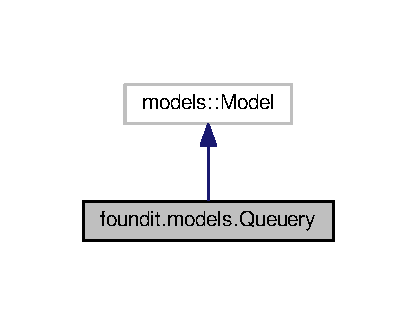
\includegraphics[width=200pt]{classfoundit_1_1models_1_1_queuery__coll__graph}
\end{center}
\end{figure}
\subsection*{Public Member Functions}
\begin{DoxyCompactItemize}
\item 
def \hyperlink{classfoundit_1_1models_1_1_queuery_a519b4c4c91400a99a5c09e89372a923c}{\+\_\+\+\_\+str\+\_\+\+\_\+} (self)
\end{DoxyCompactItemize}
\subsection*{Static Public Attributes}
\begin{DoxyCompactItemize}
\item 
\hyperlink{classfoundit_1_1models_1_1_queuery_a16c89cda1ca4f091312e152c9fac368e}{subreddit} = models.\+Char\+Field(max\+\_\+length=200)
\end{DoxyCompactItemize}


\subsection{Member Function Documentation}
\index{foundit\+::models\+::\+Queuery@{foundit\+::models\+::\+Queuery}!\+\_\+\+\_\+str\+\_\+\+\_\+@{\+\_\+\+\_\+str\+\_\+\+\_\+}}
\index{\+\_\+\+\_\+str\+\_\+\+\_\+@{\+\_\+\+\_\+str\+\_\+\+\_\+}!foundit\+::models\+::\+Queuery@{foundit\+::models\+::\+Queuery}}
\subsubsection[{\texorpdfstring{\+\_\+\+\_\+str\+\_\+\+\_\+(self)}{__str__(self)}}]{\setlength{\rightskip}{0pt plus 5cm}def foundit.\+models.\+Queuery.\+\_\+\+\_\+str\+\_\+\+\_\+ (
\begin{DoxyParamCaption}
\item[{}]{self}
\end{DoxyParamCaption}
)}\hypertarget{classfoundit_1_1models_1_1_queuery_a519b4c4c91400a99a5c09e89372a923c}{}\label{classfoundit_1_1models_1_1_queuery_a519b4c4c91400a99a5c09e89372a923c}


\subsection{Member Data Documentation}
\index{foundit\+::models\+::\+Queuery@{foundit\+::models\+::\+Queuery}!subreddit@{subreddit}}
\index{subreddit@{subreddit}!foundit\+::models\+::\+Queuery@{foundit\+::models\+::\+Queuery}}
\subsubsection[{\texorpdfstring{subreddit}{subreddit}}]{\setlength{\rightskip}{0pt plus 5cm}foundit.\+models.\+Queuery.\+subreddit = models.\+Char\+Field(max\+\_\+length=200)\hspace{0.3cm}{\ttfamily [static]}}\hypertarget{classfoundit_1_1models_1_1_queuery_a16c89cda1ca4f091312e152c9fac368e}{}\label{classfoundit_1_1models_1_1_queuery_a16c89cda1ca4f091312e152c9fac368e}


The documentation for this class was generated from the following file\+:\begin{DoxyCompactItemize}
\item 
/home/user/\+Dropbox/\+School/\+C\+S\+C\+I Stuff/\+C\+S\+C\+I 3308-\/ Software Development/\+Foundit Project/ufoundit/foundit/\hyperlink{models_8py}{models.\+py}\end{DoxyCompactItemize}

\chapter{File Documentation}
\hypertarget{____init_____8py}{}\section{/home/user/\+Dropbox/\+School/\+C\+S\+CI Stuff/\+C\+S\+CI 3308-\/ Software Development/\+Foundit Project/ufoundit/foundit/\+\_\+\+\_\+init\+\_\+\+\_\+.py File Reference}
\label{____init_____8py}\index{/home/user/\+Dropbox/\+School/\+C\+S\+C\+I Stuff/\+C\+S\+C\+I 3308-\/ Software Development/\+Foundit Project/ufoundit/foundit/\+\_\+\+\_\+init\+\_\+\+\_\+.\+py@{/home/user/\+Dropbox/\+School/\+C\+S\+C\+I Stuff/\+C\+S\+C\+I 3308-\/ Software Development/\+Foundit Project/ufoundit/foundit/\+\_\+\+\_\+init\+\_\+\+\_\+.\+py}}
\subsection*{Namespaces}
\begin{DoxyCompactItemize}
\item 
 \hyperlink{namespacefoundit}{foundit}
\end{DoxyCompactItemize}

\hypertarget{admin_8py}{}\section{/home/user/\+Dropbox/\+School/\+C\+S\+CI Stuff/\+C\+S\+CI 3308-\/ Software Development/\+Foundit Project/ufoundit/foundit/admin.py File Reference}
\label{admin_8py}\index{/home/user/\+Dropbox/\+School/\+C\+S\+C\+I Stuff/\+C\+S\+C\+I 3308-\/ Software Development/\+Foundit Project/ufoundit/foundit/admin.\+py@{/home/user/\+Dropbox/\+School/\+C\+S\+C\+I Stuff/\+C\+S\+C\+I 3308-\/ Software Development/\+Foundit Project/ufoundit/foundit/admin.\+py}}
\subsection*{Namespaces}
\begin{DoxyCompactItemize}
\item 
 \hyperlink{namespacefoundit_1_1admin}{foundit.\+admin}
\end{DoxyCompactItemize}

\hypertarget{apps_8py}{}\section{/home/user/\+Dropbox/\+School/\+C\+S\+CI Stuff/\+C\+S\+CI 3308-\/ Software Development/\+Foundit Project/ufoundit/foundit/apps.py File Reference}
\label{apps_8py}\index{/home/user/\+Dropbox/\+School/\+C\+S\+C\+I Stuff/\+C\+S\+C\+I 3308-\/ Software Development/\+Foundit Project/ufoundit/foundit/apps.\+py@{/home/user/\+Dropbox/\+School/\+C\+S\+C\+I Stuff/\+C\+S\+C\+I 3308-\/ Software Development/\+Foundit Project/ufoundit/foundit/apps.\+py}}
\subsection*{Classes}
\begin{DoxyCompactItemize}
\item 
class \hyperlink{classfoundit_1_1apps_1_1_foundit_config}{foundit.\+apps.\+Foundit\+Config}
\end{DoxyCompactItemize}
\subsection*{Namespaces}
\begin{DoxyCompactItemize}
\item 
 \hyperlink{namespacefoundit_1_1apps}{foundit.\+apps}
\end{DoxyCompactItemize}

\hypertarget{foundit_8py}{}\section{/home/user/\+Dropbox/\+School/\+C\+S\+CI Stuff/\+C\+S\+CI 3308-\/ Software Development/\+Foundit Project/ufoundit/foundit/foundit.py File Reference}
\label{foundit_8py}\index{/home/user/\+Dropbox/\+School/\+C\+S\+C\+I Stuff/\+C\+S\+C\+I 3308-\/ Software Development/\+Foundit Project/ufoundit/foundit/foundit.\+py@{/home/user/\+Dropbox/\+School/\+C\+S\+C\+I Stuff/\+C\+S\+C\+I 3308-\/ Software Development/\+Foundit Project/ufoundit/foundit/foundit.\+py}}
\subsection*{Namespaces}
\begin{DoxyCompactItemize}
\item 
 \hyperlink{namespacefoundit_1_1foundit}{foundit.\+foundit}
\end{DoxyCompactItemize}
\subsection*{Functions}
\begin{DoxyCompactItemize}
\item 
def \hyperlink{namespacefoundit_1_1foundit_a417cf87b2677c1439ee12bab5e23124e}{foundit.\+foundit.\+schedule} (subreddit, post\+Limit, top\+Com\+Limit, top\+Reply\+Limit, top\+Word\+Limit, top\+User\+Limit, oldest\+Post\+Limit, active\+Post\+Limit, wc)
\item 
def \hyperlink{namespacefoundit_1_1foundit_a8904e5a32351d54fbbc0971b30424e6c}{foundit.\+foundit.\+get\+Submission\+Age} (submission)
\begin{DoxyCompactList}\small\item\em temp=q.\+fetch\+\_\+job(jobq\mbox{[}qindex\mbox{]}).get\+\_\+id.\+result temp=q.\+fetch\+\_\+job(jobq\mbox{[}qindex\mbox{]}).id.\+result if(temp)\+: results.\+append(temp) q.\+remove(q.\+fetch\+\_\+job(jobq\mbox{[}qindex\mbox{]}).id) check+=1 gindex+=1 print(\char`\"{}\+W\+O\+R\+K\+E\+R S\+E\+A\+R\+C\+H \#\char`\"{}+str(qindex)+(\char`\"{} D\+O\+N\+E!!!\char`\"{})+\char`\"{}v\+T\+O\+T\+A\+L C\+O\+M\+P\+L\+E\+T\+E\+: \char`\"{}+str(check)) time.\+sleep(workercount+3) qindex+=1 time.\+sleep(workercount$\ast$2) print(\char`\"{}\+W\+A\+I\+T\+I\+N\+G...\char`\"{}) if(check!=workercount)\+: qindex=0 C\+O\+M\+B\+I\+NE A\+LL D\+A\+TA O\+N\+CE C\+H\+E\+CK P\+A\+S\+S\+ES O\+R\+D\+ER OF R\+E\+T\+U\+RN F\+OR W\+O\+R\+K\+E\+RS 0title\+Words, 1noun\+Dict, 2user\+Dict, 3top\+Com, 4top\+Reply, 5oldest\+Post, 6active\+Post, 7posts\+Analyzed, 8total\+Length\+All, 9comments\+Analyzed) \end{DoxyCompactList}\item 
def \hyperlink{namespacefoundit_1_1foundit_ae5d1e300e19274d4bb4c0db668d13714}{foundit.\+foundit.\+adjust} (l, limit, index\+To\+Compare, thing\+To\+Add)
\item 
def \hyperlink{namespacefoundit_1_1foundit_a0a97ddadcb8a2cc47d44c8810dc8af05}{foundit.\+foundit.\+search} (subreddit, post\+Limit, top\+Com\+Limit, top\+Reply\+Limit, top\+Word\+Limit, top\+User\+Limit, oldest\+Post\+Limit, active\+Post\+Limit, startpos, endpos, qindex)
\end{DoxyCompactItemize}
\subsection*{Variables}
\begin{DoxyCompactItemize}
\item 
\hyperlink{namespacefoundit_1_1foundit_ae9cda1f3b56d2dd4499216536e44b722}{foundit.\+foundit.\+q} = Queue(connection=conn)
\end{DoxyCompactItemize}

\hypertarget{foundit__old_8py}{}\section{/home/user/\+Dropbox/\+School/\+C\+S\+CI Stuff/\+C\+S\+CI 3308-\/ Software Development/\+Foundit Project/ufoundit/foundit/foundit\+\_\+old.py File Reference}
\label{foundit__old_8py}\index{/home/user/\+Dropbox/\+School/\+C\+S\+C\+I Stuff/\+C\+S\+C\+I 3308-\/ Software Development/\+Foundit Project/ufoundit/foundit/foundit\+\_\+old.\+py@{/home/user/\+Dropbox/\+School/\+C\+S\+C\+I Stuff/\+C\+S\+C\+I 3308-\/ Software Development/\+Foundit Project/ufoundit/foundit/foundit\+\_\+old.\+py}}
\subsection*{Namespaces}
\begin{DoxyCompactItemize}
\item 
 \hyperlink{namespacefoundit_1_1foundit__old}{foundit.\+foundit\+\_\+old}
\end{DoxyCompactItemize}
\subsection*{Functions}
\begin{DoxyCompactItemize}
\item 
def \hyperlink{namespacefoundit_1_1foundit__old_a87bf8701c89694eb3f6c6fbd11582ff5}{foundit.\+foundit\+\_\+old.\+get\+Submission\+Age} (submission)
\item 
def \hyperlink{namespacefoundit_1_1foundit__old_ab326b5587621f5ce27348998be899ff6}{foundit.\+foundit\+\_\+old.\+search} (subreddit, post\+Limit, top\+Com\+Limit, top\+Word\+Limit, top\+User\+Limit, oh\+Snap\+Limit, oldest\+Post\+Limit)
\end{DoxyCompactItemize}

\hypertarget{graph_8py}{}\section{/home/user/\+Dropbox/\+School/\+C\+S\+CI Stuff/\+C\+S\+CI 3308-\/ Software Development/\+Foundit Project/ufoundit/foundit/graph.py File Reference}
\label{graph_8py}\index{/home/user/\+Dropbox/\+School/\+C\+S\+C\+I Stuff/\+C\+S\+C\+I 3308-\/ Software Development/\+Foundit Project/ufoundit/foundit/graph.\+py@{/home/user/\+Dropbox/\+School/\+C\+S\+C\+I Stuff/\+C\+S\+C\+I 3308-\/ Software Development/\+Foundit Project/ufoundit/foundit/graph.\+py}}
\subsection*{Namespaces}
\begin{DoxyCompactItemize}
\item 
 \hyperlink{namespacefoundit_1_1graph}{foundit.\+graph}
\end{DoxyCompactItemize}
\subsection*{Functions}
\begin{DoxyCompactItemize}
\item 
def \hyperlink{namespacefoundit_1_1graph_ad382cb5cac25f52e045b61c77b3e5245}{foundit.\+graph.\+uautolabel} (rects, ax)
\item 
def \hyperlink{namespacefoundit_1_1graph_ac72321993b1a3abe0633ffb1f3ac4d08}{foundit.\+graph.\+urender\+Graph} (data\+Set)
\item 
def \hyperlink{namespacefoundit_1_1graph_a831dedc0a3b858f3c05ef6e19d45667f}{foundit.\+graph.\+render\+Graph} (data\+Set)
\end{DoxyCompactItemize}

\hypertarget{graphtest_8py}{}\section{/home/user/\+Dropbox/\+School/\+C\+S\+CI Stuff/\+C\+S\+CI 3308-\/ Software Development/\+Foundit Project/ufoundit/foundit/graphtest.py File Reference}
\label{graphtest_8py}\index{/home/user/\+Dropbox/\+School/\+C\+S\+C\+I Stuff/\+C\+S\+C\+I 3308-\/ Software Development/\+Foundit Project/ufoundit/foundit/graphtest.\+py@{/home/user/\+Dropbox/\+School/\+C\+S\+C\+I Stuff/\+C\+S\+C\+I 3308-\/ Software Development/\+Foundit Project/ufoundit/foundit/graphtest.\+py}}
\subsection*{Namespaces}
\begin{DoxyCompactItemize}
\item 
 \hyperlink{namespacefoundit_1_1graphtest}{foundit.\+graphtest}
\end{DoxyCompactItemize}
\subsection*{Variables}
\begin{DoxyCompactItemize}
\item 
list \hyperlink{namespacefoundit_1_1graphtest_a598db4fa9693ae9cc94d8ebe41d59224}{foundit.\+graphtest.\+a} = \mbox{[}1, 2\mbox{]}
\item 
list \hyperlink{namespacefoundit_1_1graphtest_add8d87bd6a6890fe6f2682f0f7990ed9}{foundit.\+graphtest.\+b} = \mbox{[}2, 5\mbox{]}
\item 
\hyperlink{namespacefoundit_1_1graphtest_aae9ec7ea98940dc46b73c2908419e44c}{foundit.\+graphtest.\+bins}
\item 
\hyperlink{namespacefoundit_1_1graphtest_a0717e136db67aedb0ff4cffd4fc30c5f}{foundit.\+graphtest.\+weights}
\end{DoxyCompactItemize}

\hypertarget{models_8py}{}\section{/home/user/\+Dropbox/\+School/\+C\+S\+CI Stuff/\+C\+S\+CI 3308-\/ Software Development/\+Foundit Project/ufoundit/foundit/models.py File Reference}
\label{models_8py}\index{/home/user/\+Dropbox/\+School/\+C\+S\+C\+I Stuff/\+C\+S\+C\+I 3308-\/ Software Development/\+Foundit Project/ufoundit/foundit/models.\+py@{/home/user/\+Dropbox/\+School/\+C\+S\+C\+I Stuff/\+C\+S\+C\+I 3308-\/ Software Development/\+Foundit Project/ufoundit/foundit/models.\+py}}
\subsection*{Classes}
\begin{DoxyCompactItemize}
\item 
class \hyperlink{classfoundit_1_1models_1_1_queuery}{foundit.\+models.\+Queuery}
\end{DoxyCompactItemize}
\subsection*{Namespaces}
\begin{DoxyCompactItemize}
\item 
 \hyperlink{namespacefoundit_1_1models}{foundit.\+models}
\end{DoxyCompactItemize}

\hypertarget{tests_8py}{}\section{/home/user/\+Dropbox/\+School/\+C\+S\+CI Stuff/\+C\+S\+CI 3308-\/ Software Development/\+Foundit Project/ufoundit/foundit/tests.py File Reference}
\label{tests_8py}\index{/home/user/\+Dropbox/\+School/\+C\+S\+C\+I Stuff/\+C\+S\+C\+I 3308-\/ Software Development/\+Foundit Project/ufoundit/foundit/tests.\+py@{/home/user/\+Dropbox/\+School/\+C\+S\+C\+I Stuff/\+C\+S\+C\+I 3308-\/ Software Development/\+Foundit Project/ufoundit/foundit/tests.\+py}}
\subsection*{Namespaces}
\begin{DoxyCompactItemize}
\item 
 \hyperlink{namespacefoundit_1_1tests}{foundit.\+tests}
\end{DoxyCompactItemize}

\hypertarget{urls_8py}{}\section{/home/user/\+Dropbox/\+School/\+C\+S\+CI Stuff/\+C\+S\+CI 3308-\/ Software Development/\+Foundit Project/ufoundit/foundit/urls.py File Reference}
\label{urls_8py}\index{/home/user/\+Dropbox/\+School/\+C\+S\+C\+I Stuff/\+C\+S\+C\+I 3308-\/ Software Development/\+Foundit Project/ufoundit/foundit/urls.\+py@{/home/user/\+Dropbox/\+School/\+C\+S\+C\+I Stuff/\+C\+S\+C\+I 3308-\/ Software Development/\+Foundit Project/ufoundit/foundit/urls.\+py}}
\subsection*{Namespaces}
\begin{DoxyCompactItemize}
\item 
 \hyperlink{namespacefoundit_1_1urls}{foundit.\+urls}
\end{DoxyCompactItemize}
\subsection*{Variables}
\begin{DoxyCompactItemize}
\item 
list \hyperlink{namespacefoundit_1_1urls_aa83b5e06599a5865f06d3d9c2d4f5a21}{foundit.\+urls.\+urlpatterns}
\end{DoxyCompactItemize}

\hypertarget{utils_8py}{}\section{/home/user/\+Dropbox/\+School/\+C\+S\+CI Stuff/\+C\+S\+CI 3308-\/ Software Development/\+Foundit Project/ufoundit/foundit/utils.py File Reference}
\label{utils_8py}\index{/home/user/\+Dropbox/\+School/\+C\+S\+C\+I Stuff/\+C\+S\+C\+I 3308-\/ Software Development/\+Foundit Project/ufoundit/foundit/utils.\+py@{/home/user/\+Dropbox/\+School/\+C\+S\+C\+I Stuff/\+C\+S\+C\+I 3308-\/ Software Development/\+Foundit Project/ufoundit/foundit/utils.\+py}}
\subsection*{Namespaces}
\begin{DoxyCompactItemize}
\item 
 \hyperlink{namespacefoundit_1_1utils}{foundit.\+utils}
\end{DoxyCompactItemize}
\subsection*{Functions}
\begin{DoxyCompactItemize}
\item 
def \hyperlink{namespacefoundit_1_1utils_a59497bd850949eb6946d3ddf7fb17d85}{foundit.\+utils.\+return\+U\+RL} (str1, str2)
\end{DoxyCompactItemize}

\hypertarget{views_8py}{}\section{/home/user/\+Dropbox/\+School/\+C\+S\+CI Stuff/\+C\+S\+CI 3308-\/ Software Development/\+Foundit Project/ufoundit/foundit/views.py File Reference}
\label{views_8py}\index{/home/user/\+Dropbox/\+School/\+C\+S\+C\+I Stuff/\+C\+S\+C\+I 3308-\/ Software Development/\+Foundit Project/ufoundit/foundit/views.\+py@{/home/user/\+Dropbox/\+School/\+C\+S\+C\+I Stuff/\+C\+S\+C\+I 3308-\/ Software Development/\+Foundit Project/ufoundit/foundit/views.\+py}}
\subsection*{Namespaces}
\begin{DoxyCompactItemize}
\item 
 \hyperlink{namespacefoundit_1_1views}{foundit.\+views}
\end{DoxyCompactItemize}
\subsection*{Functions}
\begin{DoxyCompactItemize}
\item 
def \hyperlink{namespacefoundit_1_1views_a7dd28e8760cb6ba397d734043c840841}{foundit.\+views.\+index} (request)
\item 
def \hyperlink{namespacefoundit_1_1views_a1cea187af3aaa9ac41218cd985a3f24b}{foundit.\+views.\+loading} (request)
\item 
def \hyperlink{namespacefoundit_1_1views_a91bc63c48fad0582cbcff41458970486}{foundit.\+views.\+check\+Job} (request)
\item 
def \hyperlink{namespacefoundit_1_1views_a07ba7672a02678833190150670718cae}{foundit.\+views.\+test\+Results} (request)
\item 
def \hyperlink{namespacefoundit_1_1views_aaacc45f037dbadfc5ecd92f0a1ffa4e6}{foundit.\+views.\+results} (request)
\end{DoxyCompactItemize}
\subsection*{Variables}
\begin{DoxyCompactItemize}
\item 
\hyperlink{namespacefoundit_1_1views_a933f4b14aa78ea94e74f8f93970e4b12}{foundit.\+views.\+q} = Queue(connection=conn)
\item 
string \hyperlink{namespacefoundit_1_1views_a326af97fa9bba95a26dcbb7c1a1f0f04}{foundit.\+views.\+title} = \char`\"{}\char`\"{}
\item 
int \hyperlink{namespacefoundit_1_1views_adcdd2d7a86d9c9a1d91112a22adab904}{foundit.\+views.\+workercount} = 5
\end{DoxyCompactItemize}

%--- End generated contents ---

% Index
\backmatter
\newpage
\phantomsection
\clearemptydoublepage
\addcontentsline{toc}{chapter}{Index}
\printindex

\end{document}
